\section{The breaking of the gauge group and the bosons it produces}
\label{sec:breaking}

\subsection{What ``broken'' means for a gauge group}

At a minimum with $\Delta_{U2}\neq0$ the pair field is invariant under $SU(2)_{U2}$ and changes its
phase under $U(1)_{U2}$ [Eq.~\eqref{eq:detE}]. The transformations that leave it invariant are
those with $\det\Upsilon_{U2}=1$, so the condensate breaks
\begin{equation}
U(2)_{U2}\ \to\ SU(2)_{U2},
\label{eq:breaking}
\end{equation}
with one broken generator, the phase $\theta_{U2}$ of $\Delta_{U2}=|\Delta_{U2}|\exp(i\theta_{U2})$. A local
symmetry cannot be broken spontaneously in the literal sense (Elitzur's theorem~\cite{Elitzur1975}):
without a choice of gauge, $\langle\Phi^+_{U2}\rangle$ averages to zero over the gauge orbit. The
statement ``the gauge group is spontaneously broken'' means, as for superconductors and for the
electroweak theory~\cite{Anderson1963,EnglertBrout1964,Higgs1964,GHK1964}: in a fixed gauge
$\langle\Phi^+_{U2}\rangle\neq0$; gauge-invariantly, the gauge boson of the broken generator is
massive (the Meissner effect, Sec.~\ref{sec:stiffness}), the would-be Goldstone boson is absorbed by
it, and the amplitude $|\Delta_{U2}|$ of the condensate is nonzero. The rest of this section derives
these statements and the new scalar.

\subsection{Small oscillations in the random-phase approximation}

Let the composite fields oscillate about the minimum,
$(\Delta_1,\Delta_2,M_{U2})\to(\Delta_1,\Delta_2,M_{U2})_{\min}+(\text{amplitudes})\times\exp(-iw_{U2}x4)$,
where $\Delta_1$ and $\Delta_2$ are the real and imaginary parts of $\Delta_{U2}$, and the minimum is
taken with $\Delta_2=0$. The Bogoliubov--de Gennes matrix depends on them linearly, through the
vertices $\mathsf V^1_{U2}$, $\mathsf V^2_{U2}=i\,\mathrm{diag}(\mathsf 1_{16},-\mathsf 1_{16})\mathsf V^1_{U2}$
and $\mathsf V^3_{U2}$ of Sec.~\ref{sec:spectrum}. The linearized self-consistency conditions have a
solution with nonzero amplitudes if and only if $\det\mathsf R_{U2}(w_{U2})=0$, where
\begin{equation}
\mathsf R_{U2}(w_{U2})=\mathrm{diag}\Big(\frac2{G^P_{U2}},\frac2{G^P_{U2}},\frac1{2G^S_{U2}}\Big)+\Pi_{U2}(w_{U2})
\label{eq:R}
\end{equation}
is the $3\times3$ matrix of the second derivatives of the classical part $\Omega^{\rm cl}_{U2}$ with
respect to $(\Delta_1,\Delta_2,M_{U2})$ plus the polarization $\Pi_{U2}$ of the fermions (the
random-phase approximation). Its entry in the first row and
column is
\begin{equation}
\begin{aligned}
\big[\Pi_{U2}(w_{U2})\big]_{11}={}&\int\!\frac{d^7q}{(2\pi)^7}\\
&\times\sum_{\rm o,e}\big|{}_{U2}\langle\mathrm e|\mathsf V^1_{U2}|\mathrm o\rangle_{U2}\big|^2\\
&\times\Big[\frac{1}{w_{U2}-\mathcal E^{\rm e}_{U2}+\mathcal E^{\rm o}_{U2}}\\
&\qquad-\frac{1}{w_{U2}+\mathcal E^{\rm e}_{U2}-\mathcal E^{\rm o}_{U2}}\Big],
\end{aligned}
\label{eq:Pi}
\end{equation}
summed over the occupied eigenvectors $|\mathrm o\rangle_{U2}$ (eigenvalue $\mathcal E^{\rm o}_{U2}<0$)
and the empty eigenvectors $|\mathrm e\rangle_{U2}$ (eigenvalue $\mathcal E^{\rm e}_{U2}\ge0$) of
$\mathsf H_{U2}(\vec q)$. The other entries follow by replacing, in the first term, the vertex of the
bra-ket on the left by that of the row and the one on the right by that of the column, and in the
second term the reverse. At $w_{U2}=0$, Eq.~\eqref{eq:Pi} is second-order perturbation theory for
the energy of the occupied states, so $\mathsf R_{U2}(0)$ is the Hessian of $\Omega_{U2}$ at the
minimum (R3-M3). For $G^S_{U2}=0$ the mass is frozen at $m_{U2}$ and $\mathsf R_{U2}$ is the
$2\times2$ matrix of $\Delta_1$ and $\Delta_2$.

\emph{The Goldstone mode.} Because $\Omega_{U2}$ depends on $|\Delta_{U2}|$ only, the second derivative
in the direction of the phase vanishes at the minimum: $[\mathsf R_{U2}(0)]_{22}=2/G^P_{U2}
+[\Pi_{U2}(0)]_{22}=0$, which is the gap equation in another form. The programs verify it at every
minimum computed, in the vacuum with and without a bare mass and at finite density (R3-M2, R3-M8,
R3-M9), to the accuracy of the quadrature: the oscillation of the phase has zero frequency at zero
momentum, the Goldstone mode~\cite{Nambu1960,Goldstone1961}.

\subsection{The amplitude mode $\sigma_{U2}$: a new neutral scalar}
\label{sec:sigma}

In the vacuum without scalar coupling the amplitude entry can be evaluated in closed form. At
$\mu_{U2}=0$ the eigenvalues of $\mathsf H_{U2}$ are $\pm E^+_{U2}$ with $E^+_{U2}=(q^2+s_{U2})^{1/2}$,
and the projectors on the empty and the occupied eigenvectors are
$\tfrac12(\mathsf 1_{32}\pm\mathsf H_{U2}/E^+_{U2})$. With
$\mathsf H_{U2}=\mathsf H_{U2}|_{\Delta_1=0}+\Delta_1\mathsf V^1_{U2}$, where the first part anticommutes with
$\mathsf V^1_{U2}$ and has the square $(q^2+M^2_{U2})\mathsf 1_{32}$, and with
$(\mathsf V^1_{U2})^2=\mathsf 1_{32}$, the sum in Eq.~\eqref{eq:Pi} is a trace,
\begin{equation}
\begin{aligned}
&\sum_{\rm o,e}\big|{}_{U2}\langle\mathrm e|\mathsf V^1_{U2}|\mathrm o\rangle_{U2}\big|^2\\
&=\tfrac14\mathrm{Tr}\Big[\Big(\mathsf 1_{32}+\frac{\mathsf H_{U2}}{E^+_{U2}}\Big)\mathsf V^1_{U2}\Big(\mathsf 1_{32}-\frac{\mathsf H_{U2}}{E^+_{U2}}\Big)\mathsf V^1_{U2}\Big]\\
&=\frac{16(q^2+M^2_{U2})}{(E^+_{U2})^2},
\end{aligned}
\label{eq:trace}
\end{equation}
and every excitation energy is $2E^+_{U2}$. With the gap equation in the vacuum,
$2/G^P_{U2}=16\int d^7q/(2\pi)^7/E^+_{U2}$, and with
$4(E^+_{U2})^2-4(q^2+M^2_{U2})=4|\Delta_{U2}|^2$, the amplitude entry becomes
\begin{equation}
\begin{aligned}
\big[\mathsf R_{U2}(w_{U2})\big]_{11}&=16\!\int\!\frac{d^7q}{(2\pi)^7}\,
\frac{4|\Delta_{U2}|^2-w^2_{U2}}{E^+_{U2}\,[4(E^+_{U2})^2-w^2_{U2}]}\\
&=c^\sigma_{U2}(w_{U2})\big(4|\Delta_{U2}|^2-w^2_{U2}\big),
\end{aligned}
\label{eq:sigmamass}
\end{equation}
with the positive function $c^\sigma_{U2}(w_{U2})=16\int d^7q/(2\pi)^7\,(E^+_{U2})^{-1}[4(E^+_{U2})^2
-w^2_{U2}]^{-1}$ below the threshold $2E^+_{U2}|_{q=0}$. At $\mu_{U2}=0$ the amplitude does not mix
with the phase (the mixing entry is proportional to $\mu_{U2}$), so the amplitude mode has the mass
\begin{equation}
m_{\sigma U2}=2|\Delta_{U2}|,
\label{eq:msigma}
\end{equation}
exactly, for every bare mass $m_{U2}$ and in every regularization that is used consistently in the
gap equation and in $\Pi_{U2}$ (R3-M4, R3-M12). For $m_{U2}=0$ it
sits at the pair-breaking threshold $2|\Delta_{U2}|$, as the scalar meson of Nambu and Jona-Lasinio
sits at twice the fermion mass~\cite{NJL1961} and the amplitude mode of a superconductor at twice
the gap~\cite{LittlewoodVarma1982}. For $m_{U2}>0$ the threshold is
$2(m^2_{U2}+|\Delta_{U2}|^2)^{1/2}>2|\Delta_{U2}|$: $\sigma_{U2}$ is then a \emph{bound state below the
continuum, a stable particle} (Table~\ref{tab:sigma}, Fig.~\ref{fig:modes}a). The decomposition
$4|\Delta_{U2}|^2-w^2_{U2}=(|\Delta_{U2}|^2/s_{U2})(4s_{U2}-w^2_{U2})-(m^2_{U2}/s_{U2})w^2_{U2}$ shows
why: $\Delta_1$ points partly along the radial direction of the plane of $(M_{U2},\Delta_{U2})$, whose
mode sits at the threshold $2s^{1/2}_{U2}$, and partly along the angular direction, which costs no
energy at zero frequency. At finite density, $\lambda^P_{U2}=0.5$ and $\mu_{U2}$ from 0.49 to 0.60,
the computed mass is the threshold $2|\Delta_{U2}|$ to six digits (Table~\ref{tab:density}).

The amplitude mode is the new scalar boson that the task asks for:
(i)~it is a real scalar field, the radial oscillation $|\Delta_{U2}|\to|\Delta_{U2}|_{\min}+\sigma_{U2}$
of the pair field, a Lorentz scalar because $\Phi^+_{U2}$ is one;
(ii)~it is neutral under every generator of $U(2)_{U2}$, because $|\Phi^+_{U2}|$ is gauge invariant,
and therefore under any phase that acts on the doublet as a whole; if the doublet carries no
electric charge, as assumed here (a dark sector), the pair, $B_{U2A}$ and $\sigma_{U2}$ are
electrically neutral, and the condensate is a superfluid, not a superconductor of electric charge;
(iii)~it exists only after the breaking: at $\Delta_{U2}=0$ the small oscillations of $\Phi^+_{U2}$ form
one complex field of charge 1, with two real components of equal mass, and only the minimum at
$|\Delta_{U2}|\neq0$ separates a radial direction (mass $2|\Delta_{U2}|$) from the angular one (the
Goldstone mode, absorbed by $B_{U2A}$);
(iv)~it carries the pairing interaction in the broken phase: the interaction of two fermions in the
channel of $\Phi^+_{U2}$, summed over all chains of fermion bubbles, is
\begin{equation}
\mathcal V^\sigma_{U2}(w_{U2})=-\big[\mathsf R_{U2}(w_{U2})^{-1}\big]_{11},
\label{eq:Vsigma}
\end{equation}
the propagator of $\sigma_{U2}$, whose pole is $m_{\sigma U2}$. At zero frequency it is
$-[\partial^2\Omega_{U2}/\partial\Delta_1^2]^{-1}$, negative (attractive) at every minimum tested, and
${{GENM:num_Tsigma_vac}}$ times the bare contact interaction $-G^P_{U2}/2$ at $\lambda^P_{U2}=1.05$ in
the vacuum (${{GENM:num_Tsigma_mass}}$ with $m_{U2}=0.1$, ${{GENM:num_Tsigma_den}}$ at $\mu_{U2}=0.56$,
$\lambda^P_{U2}=0.5$; R3-M11). In this precise sense the pairing in the superfluid is mediated by the
scalar $\sigma_{U2}$. It is \emph{not} the cause of the first pairing: before the breaking there is no
$\sigma_{U2}$, and the attraction that forms the condensate is the contact term $G^P_{U2}$ (or, at a
deeper level, the exchange of the $SU(2)_{U2}$ bosons, Sec.~\ref{sec:static}).

\begin{table}[t]
\caption{The amplitude mode in the vacuum with a bare mass ($\lambda^P_{U2}=1.05$, no scalar
coupling, R7, units $\Lambda_{U2}=1$): pair field at the minimum, pair-breaking threshold, computed mass
of $\sigma_{U2}$, and its ratio to $2\Delta_{U2}$, Eq.~\eqref{eq:msigma}.}
\label{tab:sigma}
\begin{ruledtabular}
\begin{tabular}{cccccc}
$m_{U2}$ & $\Delta_{U2}$ & threshold & $m_{\sigma U2}$ & $m_{\sigma U2}/2\Delta_{U2}$ & bound\\
\hline
{{ROWS:modes_mass_table}}
\end{tabular}
\end{ruledtabular}
\end{table}

\subsection{Stiffness, Meissner effect and the mass of $B_{U2A}$}
\label{sec:stiffness}

\emph{Spatial stiffness.} A condensate with a uniform phase gradient,
$\Delta_{U2}\exp(i\vec Q_{U2}\cdot\vec x)$, pairs $\psi^1_{U2}$ at $\vec q+\vec Q_{U2}/2$ with
$\psi^2_{U2}$ at $-\vec q+\vec Q_{U2}/2$. At $\mu_{U2}=0$ the eigenvalues of the corresponding
Bogoliubov--de Gennes matrix are, each eightfold (R3-C4),
\begin{equation}
\pm\Big[q^2+\tfrac14Q^2_{U2}+s_{U2}\pm\big((\vec q\cdot\vec Q_{U2})^2+|\Delta_{U2}|^2Q^2_{U2}\big)^{1/2}\Big]^{1/2}.
\label{eq:Qspec}
\end{equation}
Expanding the sum of the two branches to second order in $Q_{U2}$ and averaging
$(\vec q\cdot\vec Q_{U2})^2$ over the directions in seven dimensions, $q^2Q^2_{U2}/7$, gives the change
of the fermion term, $-2Q^2_{U2}\int d^7q/(2\pi)^7(\tfrac67q^2+M^2_{U2})(E^+_{U2})^{-3}$. In the normal
state ($\Delta_{U2}=0$) a phase gradient only shifts all momenta by $\vec Q_{U2}/2$, which cannot change
the energy; with the cutoff on $q$ it does, by the surface term
$-2Q^2_{U2}\,a^{(7)}_{U2}/[7(1+M^2_{U2})^{1/2}]$ (R3-M1: $\int_0^1q^6(\tfrac67q^2+M^2_{U2})\varepsilon^{-3}_{U2}dq
=[7(1+M^2_{U2})^{1/2}]^{-1}$), an artefact of the regularization, which we subtract. The physical
cost, $\tfrac12(f^s_{U2})^2Q^2_{U2}$, defines the spatial stiffness; for $m_{U2}=0$ (R3-M5)
\begin{equation}
(f^s_{U2})^2=4a^{(7)}_{U2}\int_0^1q^6\,\tfrac67q^2\Big[\frac1{q^3}-\frac1{(q^2+|\Delta_{U2}|^2)^{3/2}}\Big]dq>0.
\label{eq:fs}
\end{equation}

\emph{Time-like stiffness.} A phase that rotates in time, $\partial_4\theta_{U2}\neq0$, is equivalent to a
shift of the chemical potential by $-\partial_4\theta_{U2}/2$ (the pair has fermion number 2), so
$\tfrac12(f^t_{U2})^2=-\tfrac18\partial^2\Omega_{U2}/\partial\mu^2_{U2}$ at fixed $\Delta_{U2}$, i.e.\
(R3-M6)
\begin{equation}
(f^t_{U2})^2=2a^{(7)}_{U2}\int_0^1q^6|\Delta_{U2}|^2\big[(E^+_{U2})^{-3}+(E^-_{U2})^{-3}\big]dq.
\label{eq:ft}
\end{equation}
In (R7) the two differ: for small $|\Delta_{U2}|$ in the vacuum, Eqs.~\eqref{eq:fs} and \eqref{eq:ft}
give $(f^s_{U2})^2\to\tfrac97a^{(7)}_{U2}|\Delta_{U2}|^2$ and $(f^t_{U2})^2\to a^{(7)}_{U2}|\Delta_{U2}|^2$, so
$f^s_{U2}/f^t_{U2}\to(9/7)^{1/2}$; the computed ratio grows from ${{GENM:num_fsft_first}}$ at
$\lambda^P_{U2}={{GENM:num_lambda_modes_first}}$ to ${{GENM:num_fsft_last}}$ at
$\lambda^P_{U2}={{GENM:num_lambda_modes_last}}$ (Table~\ref{tab:modes}). A Lorentz-invariant vacuum must have
$f^s_{U2}=f^t_{U2}$: the difference is the Lorentz violation of the cutoff on the seven-dimensional
momentum. \emph{In (R8)} the time-like stiffness is computed from the Euclidean form of the fermion
term: $E^+_{U2}+E^-_{U2}$ is, up to a constant, the integral over the frequency $\kappa^{(4)}_{U2}$,
divided by $2\pi$, of the logarithm of
$[(\kappa^{(4)}_{U2})^2+(E^+_{U2})^2][(\kappa^{(4)}_{U2})^2+(E^-_{U2})^2]=(\kappa^2_{U2}+s_{U2}+\mu^2_{U2})^2
-4\varepsilon^2_{U2}\mu^2_{U2}$, with $\kappa^2_{U2}=q^2+(\kappa^{(4)}_{U2})^2$. The second derivative with
respect to $\mu_{U2}$ at $\mu_{U2}=0$ gives
$(f^t_{U2})^2=8\int d^8\kappa_{U2}/(2\pi)^8\,[\kappa^2_{U2}+s_{U2}-2\varepsilon^2_{U2}]/(\kappa^2_{U2}+s_{U2})^2$.
Averaged over the directions of the 8-momentum ($q^2\to\tfrac78\kappa^2_{U2}$) the numerator is
$2|\Delta_{U2}|^2-[\tfrac34\kappa^2_{U2}+s_{U2}]$; the bracket gives a part that survives at
$\Delta_{U2}=0$, i.e.\ a stiffness of the normal state, which a regularization that respects the gauge
symmetry (such as the continuation in the number of dimensions) sets to zero, exactly as the surface
term above. What remains is the same for space-like and time-like gradients, by Lorentz invariance
(R3-M7):
\begin{equation}
\begin{aligned}
f^2_{U2}&=16|\Delta_{U2}|^2\!\int_{\kappa_{U2}<1}\!\frac{d^8\kappa_{U2}}{(2\pi)^8}\frac{1}{(\kappa^2_{U2}+s_{U2})^2}\\
&=16a^{(8)}_{U2}|\Delta_{U2}|^2\int_0^1\frac{\kappa^7_{U2}\,d\kappa_{U2}}{(\kappa^2_{U2}+s_{U2})^2}.
\end{aligned}
\label{eq:fR8}
\end{equation}
Both stiffnesses are positive at every minimum: the condensate resists a twist of its phase.

\emph{The mass of $B_{U2A}$.} By Eq.~\eqref{eq:Dpair} the phase of the pair enters the effective
Lagrangian only in the gauge-covariant combination $\partial_A\theta_{U2}+g'_{U2}B_{U2A}$ (the pair has the
charge 1). In (R8),
\begin{equation}
\begin{aligned}
\mathcal L^{\rm eff}_{U2}={}&\tfrac12f^2_{U2}\,\eta^{AC}_{1671}\big(\partial_A\theta_{U2}+g'_{U2}B_{U2A}\big)\\
&\times\big(\partial_C\theta_{U2}+g'_{U2}B_{U2C}\big)+\dots
\end{aligned}
\label{eq:Leff}
\end{equation}
In the unitary gauge, $\Theta^0_{U2}=-\theta_{U2}$, the phase disappears and leaves the mass term
$\tfrac12g'^2_{U2}f^2_{U2}\,\eta^{AC}_{1671}B_{U2A}B_{U2C}$:
\begin{equation}
m_{BU2}=g'_{U2}\,f_{U2},
\label{eq:mB}
\end{equation}
the Meissner effect of $U(1)_{U2}$; the Goldstone mode becomes the longitudinal state of the massive
vector $B_{U2A}$. The three $SU(2)_{U2}$ bosons stay massless: the condensate is an $SU(2)_{U2}$
singlet, $SU(2)_{U2}$ is unbroken, and its gauge invariance forbids a mass term. Unlike the electroweak
case there is no mixing of $B_{U2A}$ with $\boldsymbol W_{U2A}$ (Sec.~\ref{sec:gauge}). In (R7) the
temporal and spatial components of $B_{U2A}$ would get the different masses $g'_{U2}f^t_{U2}$ and
$g'_{U2}f^s_{U2}$, again the Lorentz violation of that cutoff. Table~\ref{tab:modes} and
Fig.~\ref{fig:modes}b give the numbers.

\emph{The relativistic superfluid at finite density.} If $U(1)_{U2}$ were a global symmetry, the
Goldstone mode would be a sound wave with the velocity $v^G_{U2}=f^s_{U2}/f^t_{U2}$, where now
$(f^t_{U2})^2$ includes the change of $\Delta_{U2}$ with $\mu_{U2}$ (the full compressibility, which the
random-phase approximation contains). At weak coupling (R3-M10, Table~\ref{tab:density},
Fig.~\ref{fig:modes}c) two classic results hold in seven space dimensions: the whole density is
superfluid at zero temperature, $(f^s_{U2})^2=n_{U2}/(4\mu_{U2})$ (the relativistic form of Leggett's
theorem~\cite{Leggett1998,Son2002}; the factor $\tfrac14$ because the phase of the pair is twice
the phase of a fermion), within 1 per cent for $\Delta_{U2}<0.02$; and $(v^G_{U2})^2=1/7$, the sound
speed of a gas without a scale in seven space dimensions (pressure proportional to $\mu^8_{U2}$), within
1 per cent where $z_{U2}=\Delta_{U2}\,d\ln\Delta_{U2}/d\mu_{U2}<0.1$. Where the gap grows steeply with
$\mu_{U2}$ the condensation energy adds to the compressibility and lowers the velocity, roughly by
$z_{U2}^2$.

\begin{table*}[t]
\caption{Vacuum collective modes and stiffness (no scalar coupling, $m_{U2}=0$, units
$\Lambda_{U2}=1$): pair field and mass of $\sigma_{U2}$ in units of $2\Delta_{U2}$; spatial and time-like
stiffness in (R7) and their ratio; pair field and the single stiffness in (R8).
$m_{BU2}=g'_{U2}f_{U2}$.}
\label{tab:modes}
\begin{ruledtabular}
\begin{tabular}{cccccccc}
$\lambda^P_{U2}$ & $\Delta_{U2}$ & $m_{\sigma U2}/2\Delta_{U2}$ & $(f^s_{U2})^2$ (R7) & $(f^t_{U2})^2$ (R7) &
$f^s_{U2}/f^t_{U2}$ (R7) & $\Delta_{U2}$ (R8) & $f^2_{U2}$ (R8)\\
\hline
{{ROWS:modes_vacuum_table}}
\end{tabular}
\end{ruledtabular}
\end{table*}

\begin{table*}[t]
\caption{The superfluid at finite density ($\lambda^P_{U2}=0.5$, below the critical coupling of the
vacuum; $m_{U2}=0$, R7): pair field, mass of $\sigma_{U2}$ in units of the threshold $2\Delta_{U2}$,
spatial stiffness in units of $n_{U2}/4\mu_{U2}$, $z_{U2}=\Delta_{U2}\,d\ln\Delta_{U2}/d\mu_{U2}$, and the
squared Goldstone velocity in units of $1/7$.}
\label{tab:density}
\begin{ruledtabular}
\begin{tabular}{cccccc}
$\mu_{U2}$ & $\Delta_{U2}$ & $m_{\sigma U2}/2\Delta_{U2}$ & $(f^s_{U2})^2/(n_{U2}/4\mu_{U2})$ & $z_{U2}$ & $7(v^G_{U2})^2$\\
\hline
{{ROWS:modes_density_table}}
\end{tabular}
\end{ruledtabular}
\end{table*}

\begin{figure*}[t]
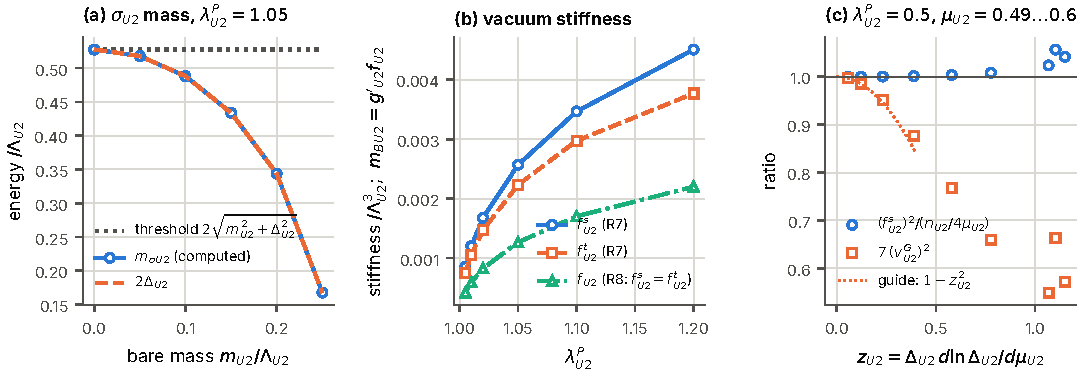
\includegraphics[width=\textwidth]{../figures/fig_r3_modes.pdf}
\caption{Collective modes (R7, no scalar coupling, units $\Lambda_{U2}=1$). (a)~Mass of $\sigma_{U2}$ in
the vacuum at $\lambda^P_{U2}=1.05$ against the bare mass: computed (circles), $2\Delta_{U2}$ (dashed) and
the pair-breaking threshold $2(m^2_{U2}+\Delta^2_{U2})^{1/2}$ (dotted); for $m_{U2}>0$ the mode is a
bound state. (b)~Vacuum stiffness against $\lambda^P_{U2}$: $f^s_{U2}$ and $f^t_{U2}$ of (R7), which differ
by the Lorentz violation of that cutoff, and the single $f_{U2}$ of (R8); $m_{BU2}=g'_{U2}f_{U2}$.
(c)~Finite density, $\lambda^P_{U2}=0.5$: $(f^s_{U2})^2/(n_{U2}/4\mu_{U2})$ and $7(v^G_{U2})^2$ against
$z_{U2}$; both are 1 at weak coupling. The dotted line $1-z^2_{U2}$ is a guide to the eye.}
\label{fig:modes}
\end{figure*}

\subsection{Static potentials between two members of the doublet}
\label{sec:static}

Two heavy (static) members of the doublet exchange the gauge bosons. In seven space dimensions a
massless vector boson gives two unit charges the potential
$V^{\rm C}_{U2}(\varrho_{U2})=\Gamma_{\rm E}(5/2)/(4\pi^{7/2}\varrho^5_{U2})$ at the distance $\varrho_{U2}$ (the
potential of a unit point charge in seven dimensions; $\Gamma_{\rm E}(5/2)=3\sqrt\pi/4$), and a
vector boson of mass $m_{BU2}$ multiplies it by
$\phi^{\rm Y}_{U2}(m_{BU2}\varrho_{U2})=\exp(-m_{BU2}\varrho_{U2})[(m_{BU2}\varrho_{U2})^2+3m_{BU2}\varrho_{U2}+3]/3$,
which solves the radial equation of the massive field in seven dimensions and equals 1 at
$\varrho_{U2}=0$ (R3-G7). Like charges repel. With the Pauli matrices $\boldsymbol\tau^{(1)}_{U2}$,
$\boldsymbol\tau^{(2)}_{U2}$ acting on the two sources,
\begin{equation}
\begin{aligned}
V^{\rm pair}_{U2}(\varrho_{U2})={}&\Big[g^2_{U2}\,\tfrac14\boldsymbol\tau^{(1)}_{U2}\cdot\boldsymbol\tau^{(2)}_{U2}
+(g'_{U2}y_{U2})^2\\
&\times\phi^{\rm Y}_{U2}(m_{BU2}\varrho_{U2})\Big]V^{\rm C}_{U2}(\varrho_{U2}),
\end{aligned}
\label{eq:Vpair}
\end{equation}
with $\tfrac14\boldsymbol\tau^{(1)}_{U2}\cdot\boldsymbol\tau^{(2)}_{U2}=-\tfrac34$ in the antisymmetric
(singlet) state of the pair and $+\tfrac14$ in the three symmetric (triplet) states (R3-B1: the sum
of the three products of Pauli matrices is twice the exchange of the two sources minus the unit).
Before the breaking ($\phi^{\rm Y}_{U2}=1$) the singlet attracts if $(g'_{U2}y_{U2})^2<\tfrac34g^2_{U2}$,
i.e.\ $(g'_{U2}/g_{U2})^2<3$; after the breaking the repulsion by $B_{U2A}$ is screened beyond the distance
$1/m_{BU2}$, while the attraction by the massless $SU(2)_{U2}$ bosons remains (Fig.~\ref{fig:static}).
The exchange of $\boldsymbol W_{U2A}$ is thus an attraction in exactly the channel of the spin-zero pair;
in this paper its effect on the gap is represented by the contact coupling $G^P_{U2}$.

\begin{figure}[t]
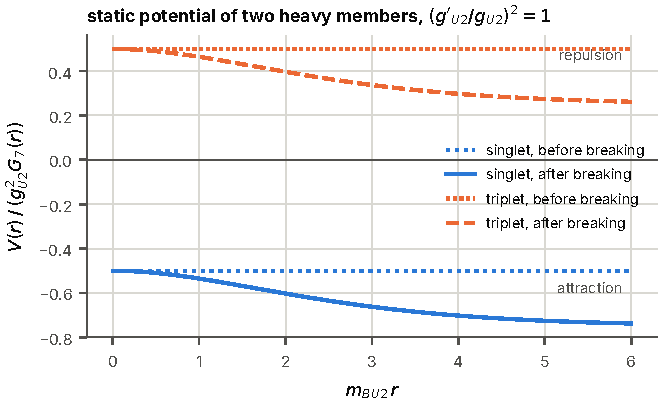
\includegraphics[width=\columnwidth]{../figures/fig_r3_static.pdf}
\caption{Static potential of two heavy members of the doublet, Eq.~\eqref{eq:Vpair}, in units of
$g^2_{U2}V^{\rm C}_{U2}(\varrho_{U2})$, for $(g'_{U2}/g_{U2})^2=1$, against $m_{BU2}\varrho_{U2}$: singlet and triplet,
before and after the breaking.}
\label{fig:static}
\end{figure}
